
\section{\app Design}

\begin{figure}[t] \centering
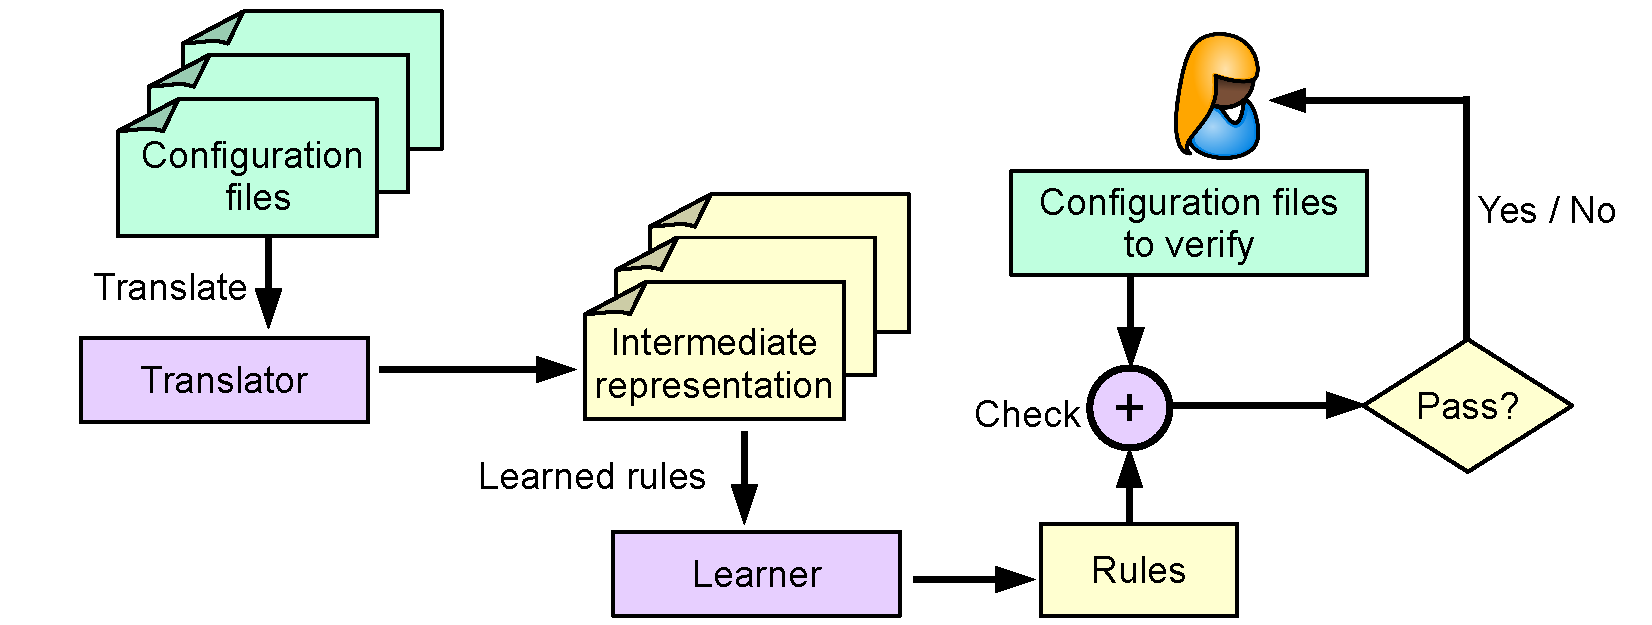
\includegraphics[width=0.8\textwidth]{figs/overview}
\caption{\app's workflow overview.}
\label{fig-overview}
\end{figure}



\xxx{
\app Design: 
  \begin{itemize}
  \item Present an architecture of \app with a fig. Briefly describe 
    how it works (step by step).
  \item Detail learner part
  \item Merge
  \item Check 
  \item Limitations
  \end{itemize}
}

\section{Learning strategy}

A primary concern in any machine learning type task is to minimize false negatives and false positives.
In the context of configuration file verification,
  a false positive is when \app reports an error on a valid confiuration file and
  a false negative is when \app fails to reports an error on an invalid confiuration file.
Too many false positives will cause users to ignore the reported error\cite{}.
However, since the cost of system failure is so high from a misconfiguration, \app propritzes the minimization of false negatives.

While a traditional classififcation learning machine learning approach can reduce both of these situations, there is can generally be no garuntee that all false negatives will be eliminated.
Instead of building classification models over the learning set (such as an SVM), we learn the largest set of rules that all correct configuration files satisfy.
In this way, \app can garuntee that, over the set of rules we consider, there will be no false negatives that could have been caught with the given learning set.
The only case of a false negative can be when there was no evidece of such a rule in the learning set - we cannot generate rules from nothing.
Framed as the question "Is this file valid", \app is complete but not sound. 

That is, taking the following definitions:
\begin{multline*}\\
\text{\{Considered Rules\}} = \forall files \in \text{\{Learning Set\}}, \{ r | r(files) = True \land r \text{ is non-trivial}\}\\
\text{\{Reported Rules\}} = {r | r(userfile)=False } \\
\text{\{True Rules\}} = \{r | \text{ if } r(userfile)=False \text{ then system crash } \land \\
   \exists file \in \text{\{Learning Set\}}, r(file) \text{ is non-trivial}\}
\end{multline*}

We have the following specification of \app.
\begin{multline*}\\
\text{\{True Rules\}} \subseteq \text{\{Considered Rules\}} \\
\forall r \in \text{\{True Rules\}}, if r(userfile)=False then \exists r \in \text{\{Reported Rules\}} \\
\neg \forall r \in \text{\{Reported Rules\}}, r \in \text{\{True Rules\}} \\
\end{multline*}

Another benefit to a rule based approach is that, unlike many classificaton models, \app can actually report the reason for failure, similar to a comiler for a programming language.
This is in contrast to neural nets for example, where we would just get a boolean value, and the mechanics of the system are entirly lost.
Reporting useful errors that specify a point of failure is important to help users fix their misconfigurations.

\section{Intermediate Representation}

Part of the reason configuration file errors are so common is because of the large number of different systems being used on the market.
Rather than proposing a new, unifying, configuration language (so that there would then be n+1 configuration languages), we use in intermediate representation language.
This allows us to reuse all our algorithms over any configuration file that can be convereted to the intermediate representation.
The portability of \app means that with very little intervtion, it can be widely used and adopted.

More grammatically complex languages tend to be harder to translation to an intermediate representation.
While there can be some context senestive structures in configuration files, we found it is easier to design the rule modules (Section \ref{}) to handle learning such structure, rather than encoding it in the intermediate representation.
Additionally, configuration files are generally grammatically simple, consisting mostly of a list of keyword-value pairs.
The keyword is the variable to be used in the system, and the value is the new value for that variable.

To specialize the converter for a particular language, a user must define a new language type, which simply acts as a flag for translation.
If a langauge requires specialized parsing, the user can write such code in the convert function based on pattern matching over the language type.
For example, the user must specify the delimiters of the language (characters for assignment and comments) for their new language. 

\section{Rules}

A core design principle in \app is modularity, so that a user can easily exentend it to their verification needs.
Rather than try to support every type of verification over configuration files, we provide a framework for defining new verfication properties.
We call each verification property a rule, for example the correct ordering of keywords or integer relationships between values.
These rules tend to be pairs of values with a relation.
For instance, an integer relation rule might be that the value of "foo" must be greater than the value of "bar".
It is also important that the rule has some empty value, to state that it is known there is no relation between the values.
This will prevent \app from trying to relearn rules when they have already been refuted.

These rules are represented as a type, where the type must support a particular interface (called a typeclass in Haskell) to be compatible with our system.
The typeclass can support anything that is Foldable, which roughly the user can use any datastructure.
In fact, in our implementation, two rules are implemented with lists, and two others use hashmaps.

\begin{lstlisting}
class Foldable t => Attribute t a where
  learn :: IRConfigFile -> t a
  merge :: t a -> t a -> t a
  check :: t a -> IRConfigFile -> Error
\end{lstlisting} 

The functions of this typeclass will be used, invisibly to the user, to make the overall system run.
As long as the specifications for each function are met, \app can garuntee completness.

\subsection{learn}
  For a single given file in the intermediate representation format, learn the full set of rules on that file.
  By overfitting to each file, we can eventually garuntee the completness of \app.
  The specification of this function is the obvious reduction of the Considered Set definition.

  $\text{learn } file =  \{ r | r(file) = True \land r \text{ is non-trivial}\}$

\subsection{merge}
  Merging the sets of rules from two files to build a new set that is true over both files is the most difficult and important function a rule must implement.
  This is generally implemented as a filter over the union of the two set, but may vary slightly.
  The formal specification of this method is that:
  \begin{multline*}
  \text{merge } Set1 \: Set2= \{r \mid \\
    r \in \text{Set1} \cup \text{Set2} \land \\
    \exists file \forall r' \in \text{Set1} \cup \text{Set2}, r(file) = True \land r'(file) = True \} \\
  \end{multline*}

\subsection{check}
  To check a file by using a rule set, we simply take all the rules that are releveant to the user's file.
  Rules that are relavent are the ones where both parts of the ordering are present.
  We learn the rule set for the user file, and every rule in the learned set must be present in the user file.

\section{Implementation}

\subsection{System}
Since we learn a set of rules on each file in isolation from the other, we have an embarrassing parallel situation.
Haskell allows us to easily take advantage of by using the parallel mapping library, parmap, both for translation to the intermediate representation, and for learning the rules on each file.
\xxx{merge can also be parallelized, but i haven't done it yet and might not get a chance}

\begin{lstlisting}
learnRules :: [ConfigFile Language] -> RuleSet
learnRules fs = let
  fs' = parMap rseq convert fs
  rs = parMap rdeepseq findAllRules fs'
 in
  foldl1 mergeRules rs
\end{lstlisting}

\subsection{Type Error Rules}
This builds a map between keywords and types, using the values as evidence.
see quantum.tex for more
i will write more on this tomorrow.

\subsection{Integer Relation Rules}
we only consider the relations , (==), (<=), (>=) because they are easy to pass aroud (as actual functions) in haskell.
We also committed cardinal since and create an instance for equality over these functions.
instance Eq (Int->Int->Bool) where

With more engineering effort, this could be extened with the use of a SMT solver to create more fine grained relational rules.
From our experience, more specific rule are not really needed for integer relations in configuration files.
However an SMT solver approach would be particularly useful for relations on strings, especially when considering substring relations between filepaths.

\subsection{Ordering and Missing Entry Rules}
These are the simpiliest of all rules, just making a lot of pairs and seeing which pairs continue to appear over the learning set.

There is actually a bit of a catch in ordering though - we are not complete over ordering rules.
This is because only our implementation does not satisfy the specification for the merge function listed above.
The problem arises from the fact the configuration files may have non-unique keywords.
Therefor, in the follwoing file we will derive the valid, but conflicting rules ([client],port) and (port,[client]).
\begin{verbatim}
[client]
port = 3306
[mysqld]
port = 3306
\end{verbatim}
Our implementation of merge removes and conflicting rules for the running set.
By introducing a renaming pass in the initial parsing we may be able to solve this, but have not found a satisfactory solution yet.
